\documentclass[a4paper]{llncs}

%\usepackage{amssymb}
%\setcounter{tocdepth}{3}
\usepackage{graphicx}

%\usepackage[linesnumbered,ruled,vlined]{algorithm2e}


\usepackage[colorlinks=true,
urlcolor=blue,
citecolor=blue,
linkcolor=blue,
           bookmarks=false,
           bookmarksnumbered,
           linktocpage=true
           ]{hyperref}

\usepackage{url}

% \urldef{\mailsa}\path|{alfred.hofmann, ursula.barth, ingrid.haas, frank.holzwarth,|
% \urldef{\mailsb}\path|anna.kramer, leonie.kunz, christine.reiss, nicole.sator,|
% \urldef{\mailsc}\path|erika.siebert-cole, peter.strasser, lncs}@springer.com|    
% \newcommand{\keywords}[1]{\par\addvspace\baselineskip
% \noindent\keywordname\enspace\ignorespaces#1}

%\usepackage{tikz}
%\usepackage{aeguill}
%\usepackage{tikzscale}
%\usepackage{filecontents} 
\usepackage{subfig}
\usepackage[font=small]{caption}

\usepackage{times}

\usepackage{color}

\newcommand{\mypara}[1]{\vspace{4pt}\noindent\textbf{#1}}
\newcommand{\mytt}[1]{\ensuremath{\mathtt{#1}}}

%% PM Define authornote command for comments
\newcommand{\authornote}[2] {
    \begin{center}
        \framebox{
            {\begin{minipage}[t]{0.9\linewidth}
                \raggedright  \textbf{[#1]}~ \scriptsize #2 \normalsize
            \end{minipage}}
    }
    \end{center}
}
\begin{document}

\mainmatter  % start of an individual contribution

% first the title is needed
\title{DataONE: A Data Federation with Provenance Support}

% \author{Yang Cao\inst{1} \and Christopher Jones\inst{2} \and V\'ictor Cuevas-Vicentt\'in\inst{3} \and Steve Aulenbach\inst{4} \and Matthew B.\ Jones\inst{2} \and Bertram Lud\"ascher\inst{1} \and Timothy McPhillips\inst{1} \and Paolo Missier\inst{5} \and  Christopher Schwalm\inst{6} \and Peter Slaughter\inst{2} \and Dave Vieglais\inst{2} \and Lauren Walker\inst{2} \and Yaxing Wei\inst{7}}

\author{Yang Cao\inst{1},  Christopher Jones\inst{2},  V\'ictor Cuevas-Vicentt\'in\inst{3},  Steve Aulenbach\inst{4},  Matthew B.\ Jones\inst{2},  Bertram Lud\"ascher\inst{1},  Timothy McPhillips\inst{1},  Paolo Missier\inst{5},   Christopher Schwalm\inst{6},  Peter Slaughter\inst{2},  Dave Vieglais\inst{2},  Lauren Walker\inst{2}, Yaxing~Wei\inst{7}}


\institute{Library and Information Science, University of Illinois, Urbana-Champaign, IL\\
\and
National Center for Ecological Analysis and Synthesis, UCSB, CA \\
\and
Universidad Popular Aut\'onoma del Estado de Puebla, Mexico\\
\and
%University Corporation for Atmospheric Research and U.S.\ Global Change Research Program \\
UCAR and U.S.\ Global Change Research Program \\
\and
School of Computing Science, Newcastle  University, UK \\
\and
Woods Hole Research Center, Falmouth, MA \\
\and
Environmental Sciences Division, Oak Ridge National Laboratory, TN}



%
% NB: a more complex sample for affiliations and the mapping to the
% corresponding authors can be found in the file "llncs.dem"
% (search for the string "\mainmatter" where a contribution starts).
% "llncs.dem" accompanies the document class "llncs.cls".
%

\toctitle{Lecture Notes in Computer Science}
\tocauthor{Authors' Instructions}
\maketitle


\begin{abstract}
  DataONE is a federated data network focusing on earth and environmental science data. We demonstrate the provenance and search features of DataONE by means of an example involving three earth scientists who interact through a DataONE MN. DataONE provenance systems enable reproducible research and facilitate proper attribution of scientific results transitively across generations of derived data products.  
  \end{abstract}

% \keywords{We would like to encourage you to list your keywords within
% the abstract section}



\section{Introduction}

Scientific workflow \emph{provenance} is valuable in computational science. Provenance can help scientists to understand their own work and share their work with others while maintaining attribution. We refer to two types of provenance: \emph{prospective} and \emph{retrospective} provenance, where the former refers to a specification of a data transformation process \cite{Freire2008}, and the latter refers to the derivations that account for the actual outcomes of one execution of the process.

DataONE (Data Observation Network for Earth) is a federated data network and a sustainable cyberinfrastructure for open, persistent, robust, and secure access to well-described and easily discovered Earth observational data~\cite{dataone}. The primary goals of DataONE are: (i) data discovery, access, integration and synthesis;  (ii) education and training, building community; and (iii) data sharing. The DataONE infrastructure consists of three principal components: (1) \emph{Member Nodes} represent existing or new data repositories that support the DataONE Member Node API; \emph{(2) Coordinating Nodes} (CN) serve the coordination and discovery needs of the network; \emph{(3) Investigator Toolkit} contains developer tools that enable programmatic interaction with DataONE infrastructure through a REST service API exposed by the CNs and MNs. 


\mypara{DataONE Search} is a web-based application that lets users seamlessly and efficiently discover publicly accessible data packages within the DataONE federated network of Member Node repositories. It allows users to search across space (geographical region), time, and using a set of keywords. Users sign in to DataONE Search using ORCID credentials, Google accounts, or institutional accounts. DataONE enables new user features like provenance-based browsing as part of its search facility. In the next section, we will demonstrate new DataONE provenance tools and the visualization of provenance with DataONE Search.


\section{Demonstration Description}  \label{demo}

In this demonstration we describe two features related to provenance. 
The first is an API for capturing \textit{retrospective} provenance from R \cite{recordr} and Matlab \cite{matlabdataone} script executions, called \emph{Run Manager}.
The second is a script annotation tool, which we call YesWorkflow \cite{yesworkflow}, designed to help developers and users better understand the structure and intent of a script.

We introduce the provenance and search features of DataONE by means of an example involving three earth scientists who interact through a DataONE MN, as shown in Fig.~\ref{fig0}.  As shown at the top of Fig.~\ref{fig0}, Alice has developed a script for producing Carbon3/Carbon4 soil maps.  She uses the YesWorkflow (YW) tool to mark-up the script and expose the underlying workflow view (i.e., prospective provenance) that is inherent in her soil mapping code as shown in Fig.\ref{fig2}. 

\begin{figure}[t] \centering 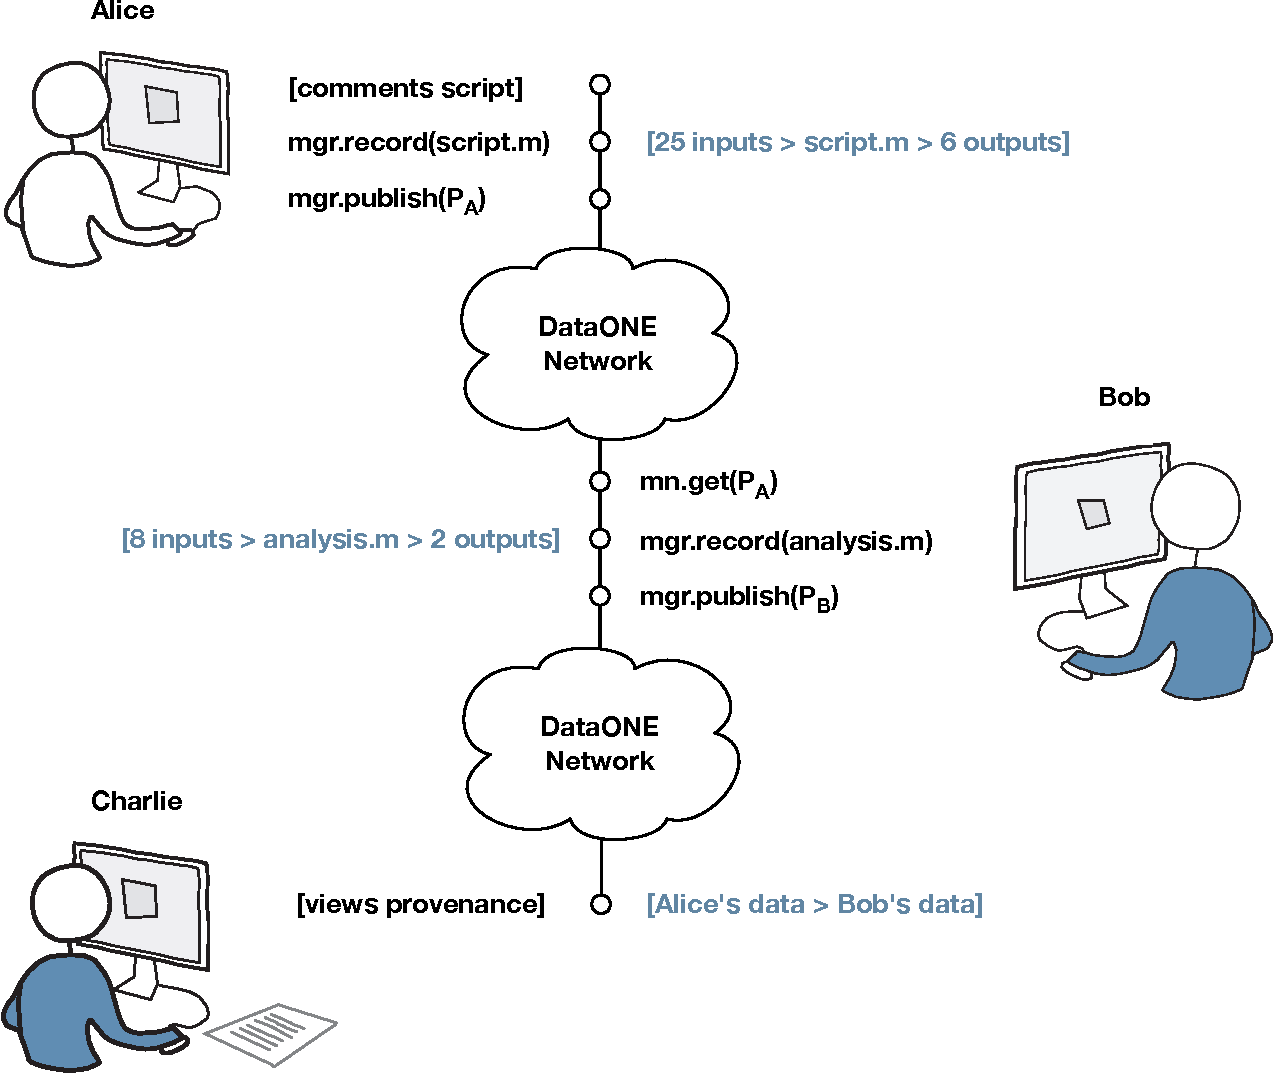
\includegraphics[width=0.4\textwidth]{figs/alice-bob-charlie-sequence-crop} \caption{Run Manager Demonstration: (1) Alice runs \mytt{script.m} with the DataONE Run Manager to create data package $P_A$, which she publishes to the DataONE network; (2) Bob later finds and downloads Alice's data, uses it in his \mytt{analysis.m}, creating and then publishing package $P_B$; (3) Charlie searches DataONE, finds Bob's $P_B$, and recognizes its dependence on Alice's $P_A$.}  \label{fig0} \end{figure}

By using the \emph{Run Manager} to run her script, Alice not only obtains the expected results, but she also captures their provenance, compliant with DataONE's ProvONE data model. 
ProvONE~\cite{provone} is an extension of the W3C PROV-O~\cite{prov-o} standard for representing provenance, and includes specializations for representing both retrospective provenance about the runtime execution and prospective provenance about the structure and flow of the analytical script or workflow.
%
At the end of the experimentation phase, Alice is ready to publish her results to a DataONE MN. 
To do so, she uses the  DataONE Matlab tool to automatically generate a DataONE-compliant data package in OAI-ORE format, including the ProvONE provenance document, the script itself, and its YW-generated workflow view. 

\begin{figure}[t]
\centering   
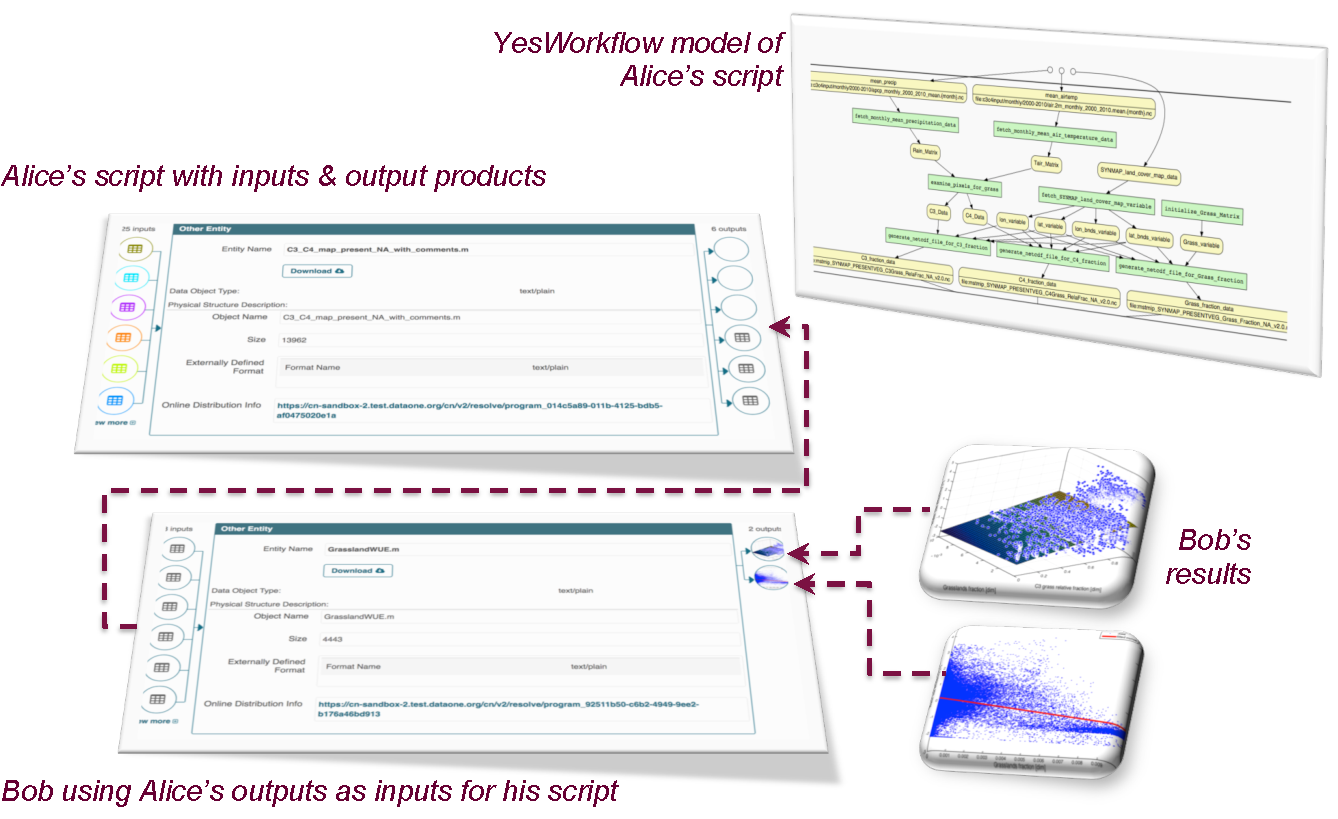
\includegraphics[width=0.8\textwidth]{figs/abc-crop}
\caption{Charlie's view on the DataONE demo site: (1) A YesWorkflow model for Alice's soil processing script; (2) Data lineage from Bob's results back through his script inputs to Alice's data package; (3) Two visualizations produced by Bob's water use efficiency analysis script.}
\label{fig2}
\end{figure}

Bob's interaction with DataONE begins with a user interface search, i.e., using the keyword ``grass'', he discovers Alice's data package, amongst others. 
He decides to use three NetCDF output data files which are part of the package, as input to his Grassland Water Use Efficiency Analysis script . 
Having identified the data of interest in the MN, Bob uses its public identifier \textit{id} to retrieve it and use it in his own code (GrasslandWUE.m).
Specifically, the \mytt{MemberNode.get}(session, id)  call, available from the Matlab Toolbox, not only correctly retrieves Alice's data package, but it also ensures that the download event is recorded as part of a new provenance document, associated to Bob's analysis.
%
Note that, if Bob create a new identifier when he downloads Alice's data, the link between two data packages would be broken, leading to a disconnect in provenance and requiring additional ``stitching'' operations~\cite{missing-link}.  

Instead, by retaining the same identifier throughout, the tool implicitly establishes a connection between Alice's work and Bob's, namely by adding a provenance statement of the form (Bob's\_execution, \emph{prov:used}, Alice's\_data\_id). Bob then proceeds to operate on the data using the DatAONE Matlab just like Alice did, eventually publishing a new data package with his own results and their provenance.
At this point, the two provenance documents are physically disjoint, as they reside in different data packages, but they are logically connected, namely through the used() statement mentioned above.
As they are both indexed by the CN upon publication of the data package, this logical connection emerges automatically when a third party, such as Charlie in our example, explores one of the two data packages.


Charlie discovers Bob's data packages on DataONE and is able to navigate back to the data that Bob used, i.e., Alice's data package depicted in Fig.~\ref{fig2}~\cite{Katz,data-trajectories}. When he searches the DataONE network using the same keyword ``grass'' from the web search interface, two data packages are displayed as shown in Fig.~\ref{fig2}, namely Alice's and Bob's. 
One data package is created by ``Alice'' \cite{yaxing}, the other is created by ``Bob'' \cite{christopher}. 

Crucially, the provenance of the two datasets is now manifested visually along with their logical connection, as shown in the DataONE Search web UI for our demo site \cite{dataone-demo} (Fig.~\ref{fig2}) and is available to Charlie. Specifically, Charlie can not only visualize the two data packages (Alice's is at the top and Bob's at the bottom), but he  is also aware of the derivation of Alice's data through Bob's script.


Provenance details for any input or output in the provenance graph can be viewed by clicking on the icon shown in the figure. DataONE Search also provides human language descriptions of how data are used or generated via the script and models, and provides navigation to ancestors and descendants in the data derivation chain. 
%
In this example, Charlie quickly learns that Alice's script (C3\_C4\_map\_present\_with\_comments.m) takes twenty-five input files and produces six outputs, shown on the left and right side of Alice's data package, respectively. The bottom three outputs in Alice's data package are the NetCDF data files that represent three different world map grids of percentage of grass types (C3 grass fraction, C4 grass fraction, and total grass fraction). In addition, a model graph is displayed at the intermediate layer that was generated by the YesWorkflow tool~\cite{yesworkflow}. Alice's used embedded YesWorkflow annotations to document her script. These annotations declare step by step how data are used and derived in the script. 

Similarly, from the provenance information associated with Bob's data package in Fig.~\ref{fig2}, we see that it takes eight inputs, and produces two visualizations. By viewing the details for each input, we can see that three of them are the outputs produced by Alice's data package.  




\section{Conclusion}

This paper demonstrates a notable new feature (provenance capture and search) of DataONE. DataONE has released the DataONE Search for public use in November 2015, and the R and Matlab provenance tool to the public in 2016. Future work of the current provenance tools include: (1) solve the broken link use case; (2) support more I/O functions; (3) handle complex scenarios such as multiple runs of a script and multiple users; (4) variable-level provenance capture warrants further investigation and efforts.
%Maintaining the link between Alice's work and Bob's subsequent work is worth discussion. Currently, Bob must use certain functions provided by DataONE to ensure the provenance link to Alice's work is correctly maintained. There are other possible ways to achieve the same goal. For example,  Bob might download Alice's data and manually add the links to Alice's work back into his data package before sharing via DataONE. A \emph{prov:was\_derived\_from} statement that local data copy for Bob is derived from Alice's data could easily add, especially for historical data for which provenance was not captured at the time data were generated.  The new provenance tools described in this demonstration allow efficient capture of machine-parseable provenance information using analytical tools commonly used in the environmental sciences (e.g., Matlab), thereby significantly improving the replicability of research in the environmental sciences.


\bibliography{references}
\bibliographystyle{splncs03}

\end{document}
